\section{Постановка задачи и численные методы её решения}
\label{sec:model}

\subsection{Модель филаментации лазерных импульсов}

В данной работе рассматривается как нестационарная задача распространения пучков (гл. \ref{sec:beams}),
так и стационарная задача распространения мощных субпикосекундных импульсов в воздухе (гл. \ref{sec:pulses}),
где необходимо учитывать дисперсию и раздельное взаимодействие импульса с компонентами воздуха при плазмообразовании.
Рассмотрим математическую постановку задачи в наиболее общем виде и последовательно сведём её
к системам уравнений для конкретных случаев.


Распространение лазерных импульсов в прозрачной среде описывается уравнением
для медленно меняющейся амплитуды электрического поля E \cite{AkhmanovVislouhChirkin, VinogradovaRudenkoSuhorukov},
являющегося следствием системы уравнений Максвелла в прозрачной среде
с керровской нелинейностью и самонаведенной лазерной плазмой:

\begin{align}\label{ModelComplexEquation}
2 i k_0 \dfrac{\partial E}{\partial z} = \left(1-\dfrac{i}{\omega_0}\dfrac{\partial}{\partial t}\right)^{-1}\Delta_{\perp}E
- \left( k_0 k'' \dfrac{\partial^2 E}{\partial t^2}
+ \sum\limits_{n = 3}^{\infty} \dfrac{1}{(i^n n!)} \left.\dfrac{\partial^n k}{\partial \omega^n}\right|_{\omega_0} \dfrac{\partial^n E}{\partial t^n}\right) + \nonumber \\
+ \dfrac{2 k_0^2}{n_0}\left[\left(1-\dfrac{i}{\omega_0}\dfrac{\partial}{\partial t}\right)\Delta n_k +
\left(1-\dfrac{i}{\omega_0}\dfrac{\partial}{\partial t}\right)\mathrm{Re}(\Delta n_p) + \mathrm{Im}(\Delta n_p)\right]E - i k_0 \alpha E.
\end{align}

В этой формуле используются следующие обозначения: $\Delta_{\perp} = \dfrac{\partial^2}{\partial x^2} + \dfrac{\partial^2}{\partial y^2}$,
$\Delta n_k$ и $\Delta n_p$ "--- добавки к показателю преломления, связанные с керровской и плазменной нелинейностями соответственно:

\begin{eqnarray}\label{ModelNkerr}
\Delta n_k(\vec{r}, z, t) & = & \frac{1}{2}n_2 I(\vec{r}, z, t) \\
\Delta n_p(\vec{r}, z, t) & = & -\frac{\omega_p^2}{2 n_0 (\omega_0^2 + \nu_c^2(\vec{r}, z, t))} 
\left(1 - i \frac{\nu_c(\vec{r}, z, t)}{\omega_0} \frac{\omega_p^2}{\omega_0^2 + \nu_c^2(\vec{r}, z, t)}\right).
\end{eqnarray}

Здесь $\omega_p = \frac{4 \pi N_e(\vec{r}, t) e^2}{m_e}$ "--- плазменная частота,
$\omega_0$ "--- центральная частота лазерного излучения,
$\nu_c$ "--- частота соударений электрона с молекулами среды, $N_e$ "--- концентрация свободных электронов,
$m_e$ "--- масса электрона, $I(\vec{r}, z, t) = \frac{c_0 n_0 \varepsilon_0}{2}|E(\vec{r}, z, t)|^2$ "--- интенсивность поля,
$c_0$ "--- скорость света в воздухе, $\varepsilon_0 = 8.85 \cdot 10^{-12}\textrm{ Ас/Вм}$ "--- электрическая постоянная.
Именно за счёт того, что знак плазменной нелинейности противоположен знаку керровской нелинейности,
возможно динамическое равновесие этих двух эффектов в~некоторой области пространства вдоль
оси распространения импульса. Оператор~$\dfrac{i}{\omega_0}\dfrac{\partial}{\partial t}$
соответствует поправкам следующего порядка к уравнению для медленно меняющейся амплитуды поля и называется оператором волновой нестационарности.


Поскольку в воздухе частота упругих столкновений электронов с молекулами компонент воздуха существенно меньше
лазерной частоты, а именно при характерной интенсивности в филаменте $5 \cdot 10^{13}\textrm{ Вт}/\textrm{см}^2$
частота столкновений $\nu_c = 4 \cdot 10^{12}\textrm{ с}^{-1}$, то есть $\nu_c \ll \omega_0 \simeq 10^{15}\textrm{ c}^{-1}$,
то добавку в показатель преломления $\Delta n_p$ можно записать в виде:

\begin{equation}\label{ModelNplasma}
\Delta n_p(\vec{r}, z, t) = -\frac{\omega_p^2}{2 n_0 \omega_0^2}
\end{equation}

Первое слагаемое в правой части (\ref{ModelComplexEquation}) описывает дифракцию пучка,
второе в скобках "--- дисперсию лазерного импульса во втором и высших приближениях теории дисперсии,
третье "--- изменение показателя преломления среды под воздействием плазменной и керровской нелинейностей.
Последнее слагаемое описывает поглощение энергии поля за счёт нелинейной ионизации молекул воздуха,
где коэффициент поглощения выражается следующим образом:

\begin{equation}\label{ModelAlphaIon}
\alpha = \sum_i \frac{m_i \hslash \omega_0}{I} \dfrac{\partial N_{ei}(\vec{r}, z, t)}{\partial t},
\end{equation}


\noindent где число $m_i$ определяют число фотонов, необходимых для ионизации молекул i-ой компоненты воздуха.
Суммирование проводится по всем компонентам воздушной смеси.


Концентрация электронов, входящая в выражение для плазменной нелинейности,
зависит от времени следующим образом:

\begin{equation}\label{ModelNe}
\dfrac{\partial N_{ei}}{\partial t} = R(I)(N_{0i} - N_{ei})
\end{equation}

Множитель $R(I)$ в правой части описывает скорость ионизации среды под действием мощного излучения,
о модели которой будет рассказано ниже; $N_{0i}$ "--- плотность нейтральных молекул среды,


\subsection{Модель нелинейной ионизации}

Рассмотрим вопрос об учёте нелинейной ионизации при рассмотрении филаментации лазерных импульсов.
Ионизация является тем механизмом, который вызывает дефокусировку импульса при сильном усилении интенсивности
вследствие керровской самофокусировки. Именно благодаря балансу между этими двумя физическими эффектами
возможно продолжительное существование плазменного канала и области высокой плотности лазерной энергии.


В общем случае при распространении мощного излучения нужно учитывать следующие процессы: многофотонную и/или туннельную ионизацию,
ударную ионизацию, и~ударно-радиационную рекомбинацию. Как было сказано выше, при определении вклада лазерной плазмы
$\Delta n_{pl}$ в нелинейный показатель преломления в воздухе можно пренебречь частотой упругих столкновений электронов
с молекулами воздуха по сравнению с частотой излучения. Таким образом, для расчёта концентрации плазмы достаточно
использовать уравнения вида (\ref{ModelNe}). Одним из первых вопрос нахождения скорости ионизации, участвующей в этом уравнении,
поднял в 1964\,г. Л.В. Келдыш \cite{Keldysh1964}. Им был введён параметр адиабатичности:

\begin{equation}
\gamma = \frac{\omega}{\omega_t} = \frac{\omega \sqrt{2 m E_i}}{e E} = \frac{1}{2 K_0 F},
\end{equation}

\noindent где $E_i$ "--- потенциал ионизации атомного уровня, $E$ "--- амплитуда электрического поля,
$F = E/E_a$ "--- приведённое поле, $K_0 = E_i/\hbar\omega$ "--- параметр многоквантовости процесса.
Было показано, что если $\gamma \gg 1$, то ионизация носит многофотонный характер, а если $\gamma \ll 1$, то туннельный.


На данный момент наиболее популярными моделями для определения скорости туннельной ионизации являются
модель Переломова-Попова-Терентьева \cite{PPT1966} и модель Аммосова-Делоне-Крайнова \cite{ADK1986}.
Как указывается в \cite{Popov2004}, формула АДК выводится из формулы ППТ при определённых приближениях, а именно в предположении ионизации
водородоподобного атома в основном состоянии, и является асимптотически точной в~пределе слабого поля. Для использования обеих формул
необходимы экспериментальные данные по скорости ионизации для нахождения эффективного заряда иона в~случае модели АДК
и эффективных квантовых чисел для модели ППТ.

%%%%%%%%%%%%%%%%%%%%%%%%%%%%%%%%%%%%%%%%

\begin{figure}[H]
    \begin{center}
        \begin{minipage}{\minipagewidthtwo}
            \center{\includegraphics[width=0.95\linewidth]{model/ionization/l800/All}}
        \end{minipage}
        \hfill        
        \begin{minipage}{\minipagewidthtwo}
            \center{\includegraphics[width=0.95\linewidth]{model/ionization/l10000/All}}
        \end{minipage}
        \\[1ex]
        \caption{Скорость ионизации $O_2$ и $N_2$ по модели ППТ для длины волны 800 нм (слева) и по модели АДК для длины волны 10 микрон (справа) в зависимости от интенсивности излучения.}
        \label{fig:ModelIonizationRates}
    \end{center}
\end{figure}

%%%%%%%%%%%%%%%%%%%%%%%%%%%%%%%%%%%%%%%%

Мною для моделирования использовались уже имеющиеся в расопряжении лаборатории данные для скорости ионизации по модели ППТ при $\lambda = 800$~нм
(так как для характерных интенсивностей в филаменте $I \simeq 5 \cdot 10^{13} \textrm{ Вт}/\textrm{см}^2$ параметр $\gamma_{\lambda=800} \sim 1$
и модель ППТ хорошо описывает эту промежуточную область)
и рассчитанные мной по модели АДК (хорошо описывает туннельную ионизацию при таких же интенсивностях) скорости ионизации для для длины волны 10 мкм.
Согласно этой модели скорость ионизации газа полем лазерного импульса выглядит следующим образом:

\begin{equation}\label{ModelADK}
R_{ADK}(I) = \sqrt{\dfrac{3 n^{*3} F}{\pi Z^3}}\dfrac{F D^2}{8 \pi Z} \exp \left( -\dfrac{2 Z^3}{3 n^{*3} F}\right),
\end{equation}

\noindent где $n^{*} = Z^{*}/\sqrt{2 E_i}$ "--- эффективной главное квантовое число, $Z^{*}$ "--- эффективный заряд иона, $E_i$ "--- безразмерный потенциал ионизации (энергия связи),
$D = \left( \dfrac{4 e Z^{*3}}{F n^{*4}} \right)^{n^{*}}$, а $F = \sqrt{I/I_a}$, где $I_a$ "--- напряжённость атомного поля. Таким образом,
скорость ионизации различных газов зависит от энергии связи $E_i$ и эффективного заряда иона $Z^{*}$. Использовались следующие значения:
$E_{i,N_2} = 15.576$~эВ, $Z^{*}_{N_2} = 0.9$, $E_{i,O_2} = 12.063$~эВ, $Z^{*}_{O_2} = 0.53$.
Используемые зависимости скорости ионизации от интенсивности лазерного излучения приведены на рис.~\ref{fig:ModelIonizationRates}.


\subsection{Методика численного моделирования}

Для задач, рассматриваемых в следующих главах, влияние дисперсии высших порядков не учитывалось,
поэтому уравнение (\ref{ModelComplexEquation}) можно было упростить до следующего вида:

\begin{equation}\label{ModelSimplifiedEquation}
2 i k_0 \dfrac{\partial E}{\partial z} = \Delta_{\perp}E - k_0 k'' \dfrac{\partial^2 E}{\partial t^2}
+ \dfrac{2 k_0^2}{n_0}\left(\Delta n_k + \Delta n_p\right)E - i k_0 \alpha E
\end{equation}

При этом $\Delta n_k$ вычисляется по формуле (\ref{ModelNkerr}), а $\Delta n_p$ "--- по формуле (\ref{ModelNplasma}).
Для численного решения уравнения (\ref{ModelSimplifiedEquation}) перейдём к безразмерным переменным:

\begin{equation}
\tilde{z} = \frac{z}{L_{diff}}, \tilde{t} = \frac{t}{\tau_0}, \tilde{r} = \frac{r}{a_0}, \tilde{E} = \frac{E}{E_0}, \tilde{N_{ei}} = \frac{N_{ei}}{N_{0i}}
\end{equation}

Подставляя выражения старых переменных через новые в (\ref{ModelSimplifiedEquation})--(\ref{ModelNe}) и опуская в записи тильды, получаем:

\begin{equation}\label{ModelNodim}
2 i \dfrac{\partial E}{\partial z} = \Delta_{\perp}E - \dfrac{L_{diff}}{L_{disp}} \dfrac{\partial^2 E}{\partial t^2} + R |E|^2 E - R_{I} N_{e} E - i \alpha E
\end{equation}

\begin{equation*}
\begin{array}{rcl}
R & = & R_{cr} \frac{P_0}{P_{cr}} \\[1.0ex]
R_{I} & = & \frac{N_0 e^2 a_0^2}{n_0 c^2 \varepsilon_0 m_e} \\[1.0ex]
\dfrac{\partial N_{e,O}}{\partial t} & = & R_{O}(I)(0.21 - N_{e,O}) \\[1.0ex]
\dfrac{\partial N_{e,N}}{\partial t} & = & R_{N}(I)(0.78 - N_{e,N}) \\[1.0ex]
N_{e} & = & N_{e,O} + N_{e,N}
\end{array}
\end{equation*}

Здесь $L_{diff} = k_0 a_0^2$ "---дифракционная длина, $L_{disp} = \frac{\tau_0^2}{|k''|}$ "--- дисперсионная длина во~втором приближении теории дисперсии.


Уравнение (\ref{ModelNodim}) решалось  с помощью метода расщепления по физическим факторам.
В соответствии с этим методом уравнение (\ref{ModelNodim}) заменяется тремя уравнениями,
каждое из которых решается на n-ом шаге вдоль координаты $z$:

\begin{enumerate}
    \item дифракционное уравнение: \\
    \begin{equation}\label{ModelNodimDiffraction}
    2 i \dfrac{\partial E}{\partial z} = \Delta_{\perp}E
    \end{equation}

    \item дисперсионное  уравнение: \\
    \begin{equation}\label{ModelNodimDispersion}
    2 i \dfrac{\partial E}{\partial z} = - \dfrac{L_{diff}}{L_{disp}} \dfrac{\partial^2 E}{\partial t^2}
    \end{equation}

    \item нелинейное уравнение, учитывающее керровскую и плазменную нелинейности, а~также потери энергии на нелинейную ионизацию: \\
    \begin{equation}\label{ModelNodimNonlinearity}
    2 i \dfrac{\partial E}{\partial z} = R |E|^2 E - R_{I} N_{e} E - i \alpha E
    \end{equation}
\end{enumerate}

При решении этой цепочки уравнений в качестве начальных условий для первого уравнения берётся поле с предыдущего шага,
а в качестве начальных условий для последующих уравнений "--- результат решения предыдущего.
Решение последнего уравнения принимается за искомый результат. Для решения однотипных уравнений дифракции и~дисперсии
использовались метод на основе неявных схем (см. \ref{subsec:AppVarXZ}--\ref{subsec:AppVarRZ}) и метод на~основе преобразования Фурье (см. \ref{subsec:AppFourier}).
Уравнение (\ref{ModelNodimNonlinearity}) является локальным по~поперечным координатам и его решение не представляет сложности:

\begin{equation}
E(\vec{r}, z + \Delta z, t) = E(\vec{r}, z, t) \cdot \exp\left( -\frac{i}{2} \left(R |E|^2 - R_{I} N_{e} - i \alpha \right) \Delta z \right)
\end{equation}


\subsection{Причины необходимости использования параллельных вычислений и~способы снижения вычислительных затрат}
Основные проблемы численного моделирования задачи филаментации лазерных импульсов связаны с многомасшабностью задачи.
Поперечные масштабы пучка примерно на два порядка превосходят возникающие в нем структуры.
В то же время размер расчётной сетки должен на порядок превосходить радиус пучка, чтобы границы сетки не отсекали существенные части пучка,
а также чтобы иметь некоторую <<буферную область>>, в которую могла бы расширяться низкоинтенсивная периферийная часть пучка,
которая существенно влияет на процесс распространения филамента \cite{KandidovShlenovKosarevaReview2009}.
В~противном случае также неизбежно возникновение краевых эффектов, приводящих к искажению решения.
На диаметр филамента должно приходиться достаточное количество точек (не~менее~10), иначе резкие перепады интенсивности в окрестности филамента
будут содержать слишком высокие пространственные частоты, что приведёт к невыполнению критерия Найквиста, наложению частот и, как следствие, неадекватности получаемого решения.
Как показывает практика, этот фактор является важным не только для~метода решения, основанного на преобразовании Фурье, но и для остальных методов.


Таким образом, количество точек в поперечном сечении может достигать $10^4$ по~каждой поперечной координате.
Количество временных слоев должно быть порядка $10^3-10^4$, а значит общее количество точек достигает величины порядка $10^{12}$,
а потребность в оперативной памяти "--- величины до 100~Гб. Даже в случае рассмотрения пучков, где временная координата не используется,
при изучении сложных пространственных структур объём данных для одного шага по $z$ доходит до 8~Гб. Это приводит к необходимости использовать для вычислений
кластерные вычислительные системы, так как только их применение позволяет обрабатывать такие объёмы данных за приемлемое время.


Но, к сожалению, не всегда есть возможность выполнять вычисления на суперкомпьютерах, и в этом случае является актуальной
задача создание более эффективной расчётной схемы. Для этого можно предложить использование неравномерных сеток, как по поперечным координатам,
так и по временной в случае исследования распространения импульсов. При исследовании различия в процессе филаментации импульсов
различных длин волн (гл. \ref{sec:pulses}) применялась следующая расчётная сетка: область изменения каждой переменной разбивалась на зоны от начала координат к краям сетки,
и в каждой следующей зоне шаг сетки увеличивался в 2 раза. Минимальное значение шага было в центральной зоне, где располагалась основная энергия импульса.
Использование неравномерной сетки автоматически приводит к выбору в качестве метода решения уравнений дифракции и дисперсии метод на основе разностных схем.

В случае, когда мощность импульса невелика по сравнению с критической мощностью самофокусировки,
и при распространении импульса возникает только один осесимметричный филамент на оси импульса, возможно уменьшить число измерений
за~счёт введения цилиндрических координат. В этом случае

\begin{equation}
\Delta_{\perp x,y} = \dfrac{\partial^2}{\partial x^2} + \dfrac{\partial^2}{\partial y^2} =
\dfrac{1}{r}\dfrac{\partial}{\partial r}\left(r\dfrac{\partial}{\partial r}\right) + \dfrac{1}{r^2}\dfrac{\partial^2}{\partial \varphi^2} =
\simeq \dfrac{1}{r}\dfrac{\partial}{\partial r}\left(r\dfrac{\partial}{\partial r}\right),
\end{equation}

\noindent а уравнение (\ref{ModelNodim}) принимает вид:

\begin{equation}\label{ModelSimplifiedEquationAxial}
2 i \dfrac{\partial E}{\partial z} = \dfrac{1}{r}\dfrac{\partial}{\partial r}\left(r\dfrac{\partial E}{\partial r}\right)
- \dfrac{L_{diff}}{L_{disp}} \dfrac{\partial^2 E}{\partial t^2} + R |E|^2 E - R_{I} N_{e} E - i \alpha E
\end{equation}

Этот способ уменьшения вычислительных затрат также был применён при рассмотрении задачи о распространении лазерного импульса в воздухе,
что позволило снизить количество точек расчётной сетки до $10^7\textrm{ -- }10^8$. Для получения консервативной схемы, в которой не возникает ложных источников поля,
связанных с неравномерным шагом, в работе применяется вариационный подход (см. \ref{subsec:AppVarRZ}).


\subsection{Апробация численных схем}

В качестве теста для программ численного решения поставленных задачи были проведены расчёты для начальных условий,
при которых уравнение квазиоптики решается аналитически. Для гауссова пучка можно получить следующее решение:

\begin{equation}
E(\vec{r}, z) =  \frac{E_0}{1 + z/iL_{diff}} \cdot \exp\left(\frac{x^2 + y^2}{2 a_0^2(1 + z/iL_{diff})} - ikz\right),
\end{equation}

\noindent или для интенсивности на оси пучка:

\begin{equation}
I(\vec{r} = 0, z) = \frac{I_0}{1 + z^2/L_{diff}^2}.
\end{equation}

Для проверки соответствия численных расчётов теоретической формуле были проведены
вычисления для различного количества точек на сетке: $N = 1024, 2048, 4096, 8192$. Степени
двойки брались из соображения наилучшего ускорения при использовании быстрого преобразования
Фурье для решения  уравнения квазиоптики на равномерной сетке.
Большое количество точек связано с тем, что для проводимых вычислительных экспериментов
с амплитудно-модулированными гауссовыми пучками необходимо удерживать большое количество Фурье-гармоник.
Во время тестов выбирался шаг по $z$ такого же порядка, как и в исследовательских расчётах
и смотрелось, на каком расстоянии результаты теоретического и численного расчётов начинают существенно различаться.

%%%%%%%%%%%%%%%%%%%%%%%%%%%%%%%%%%%%%%%%

\begin{figure}[H]
    \begin{center}
        \begin{minipage}{\minipagewidthtwo}
            \center{\includegraphics[width=0.95\linewidth]{model/test_beams_intensity/graph}}
        \end{minipage}
        \\[1ex]
        \caption{Зависимость пиковой интенсивности в пучке от пройденного расстояния.
                 Тест для программы решения уравнения дифракции, использующей метод на основе преобразования Фурье.
                 Pазмер сетки составлял 10 радиусов пучка, $N = 4096$.}
        \label{fig:ModelTestIntensity}
    \end{center}
\end{figure}

%%%%%%%%%%%%%%%%%%%%%%%%%%%%%%%%%%%%%%%%

Как видно на рис. \ref{fig:ModelTestIntensity}, видимая на глаз ошибка возникает только при $z \geq 5 L_{diff}$,
при том что за это время было пройдено 50000 шагов по $z$. Этой точности достаточно для проведения вычислительного эксперимента.
Основной вклад в эту ошибку вносит особенность метода Фурье, в котором расчётная область периодизируется
и пучок начинает интерферировать со своими копиями в соседних <<виртуальных>> областях. При проведении эксперимента
влияние этого эффекта удалось уменьшить за счёт введения искусственного затухания в периферийных областях расчётной области.

Вторым тестом была проверка формулы Марбургера \cite{DawestMarburger1969} для расстояния до нелинейного фокуса пучка,
полученная обобщением результатов численных расчётов и хорошо согласующаяся с экспериментом.
Согласно ей расстояние от плоскости z = 0 до точки, где интенсивность превышает начальную
в 10 раз (такую величину превышения использовал Марбургер при определении нелинейного фокуса) выражается формулой:

\begin{equation}\label{ModelMarburgerDim}
z_{fil} = \dfrac{0.367 L_{diff}}{\left( \left( \sqrt{\dfrac{P_0}{P_{cr}}} - 0.852 \right)^2 - 0.0219 \right)^{1/2}}
\end{equation}

В используемых безразмерных переменных эта формула имеет вид:

\begin{equation}\label{ModelMarburgerModim}
z_{fil} = \dfrac{0.367}{\left( \left( \sqrt{\dfrac{R}{R_{cr}}} - 0.852 \right)^2 - 0.0219 \right)^{1/2}},
\end{equation}

\noindent где $R_{cr}$ "--- критический параметр нелинейности, зависящий от формы импульса.
Так, для гауссового импульса $R_{cr}^{Gauss} \simeq 3.77$, а минимальное значение $R_{cr}^{Townes} \simeq 3.72$
принимает для солитонного решения "--- моды Таунса \cite{ChiaoGarmireTownes1964}.

%%%%%%%%%%%%%%%%%%%%%%%%%%%%%%%%%%%%%%%%

\begin{figure}[H]
    \begin{center}
        \begin{minipage}{\minipagewidthtwo}
            \center{\includegraphics[width=0.95\linewidth]{model/test_beams_marburger/graph}}
        \end{minipage}
        \\[1ex]
        \caption{Зависимость расстояния до нелинейного фокуса от параметра $R$, сравнение с формулой Марбургера.
                 Тест для программы решения уравнения дифракции, использующей метод на основе преобразования Фурье.
                 Pазмер сетки составлял 10 радиусов пучка, $N = 4096$.}
        \label{fig:ModelTestMarburger}
    \end{center}
\end{figure}

%%%%%%%%%%%%%%%%%%%%%%%%%%%%%%%%%%%%%%%%

Коэффициент детерминации $\rho^2 \equiv \frac{\sum_i (z_{fil,i}^{Experiment} - z_{fil,i}^{Marburger})^2}{\sum_i z_{fil,i}^{Experiment} - \bar{z}_{fil,i}^{Experiment}}$ между формулой и полученными результатами получился равным 0.993,
что даёт основания считать используемый алгоритм пригодным для численного решения уравнения (\ref{ModelNodim}) при выбранных параметрах сетки.

%%%%%%%%%%%%%%%%%%%%%%%%%%%%%%%%%%%%%%%%

\begin{figure}[H]
    \begin{center}
        \begin{minipage}{\minipagewidthtwo}
            \center{\includegraphics[width=0.95\linewidth]{model/test_impulses_marburger/graph}} \\
            \footnotesize{(а)}
        \end{minipage}
        \hfill
        \begin{minipage}{\minipagewidthtwo}
            \center{\includegraphics[width=0.95\linewidth]{model/test_impulses_energy/graph}} \\
            \footnotesize{(б)}
        \end{minipage}
        \\[1ex]
        \caption{Результаты тестов программы для расчёта распространения импульсов, использующей метод на основе разностных схем.
                 Проверялось соответствие формуле Марбургера (а) и сохранение полной энергии импульса при распространении (б).}
        \label{fig:ModelTestImpulses}
    \end{center}
\end{figure}

%%%%%%%%%%%%%%%%%%%%%%%%%%%%%%%%%%%%%%%%

Тесты на точность были также  проведены для программы, использующейся для решения уравнения квазиоптики метод на основе разностных схем.
Как видно из рис. \ref{fig:ModelTestImpulses}.а, имеется довольно хорошее соответствие. Небольшая систематическая ошибка связана с тем,
что в вычислительном эксперименте положение нелинейного фокуса определялось по точке 50-кратного увеличения интенсивности.
Кроме проверки формулы Марбургера и уменьшения пиковой интенсивности импульса при наличии дифракции и дисперсии второго порядка
в вычислительных экспериментах также контролировалась полная энергия импульса. Результаты этого теста представлены на рис. \ref{fig:ModelTestImpulses}.б.
Как видно, энергия сохраняется с точностью до $10^{-5}$ от первоначального значения. Кроме того, небольшую ошибку вносит
численное интегрирование интенсивности при использовании неравномерной неравномерной сетки.
